\section{Visualization and Visual Analytics}
Computer-based visualization systems provide visual representations of datasets designed to help people carry out tasks more effectively~\cite{Munzner2014}. Because the design space of possible visual ``idioms'' is huge, it is challenging to create effective visualizations. Understanding well-established information design principles and interaction techniques could guide designers toward the right direction. Also, every visualization needs to be evaluated to check whether it meets its design purposes and how it helps or hinder users.

\subsection{Overview}
TODO: Overview of vis and VA

%What is vis? Classic example. What vis can help from cognition (Ben) and Wijk, Fekete?
%
%Large datasets -> simple aggregation, reduction like filtering, interaction, ; larger datasets, more sophiscated emthods extract patterns and vis to display them. and allow further. That is the idea of visual analytics. Orginal def, new def. Model.
%
%Describe visual analytics process model (Figure~\ref{fig:visual-analytics-process})
%
%\begin{figure}[!htb]
%	\centering
%	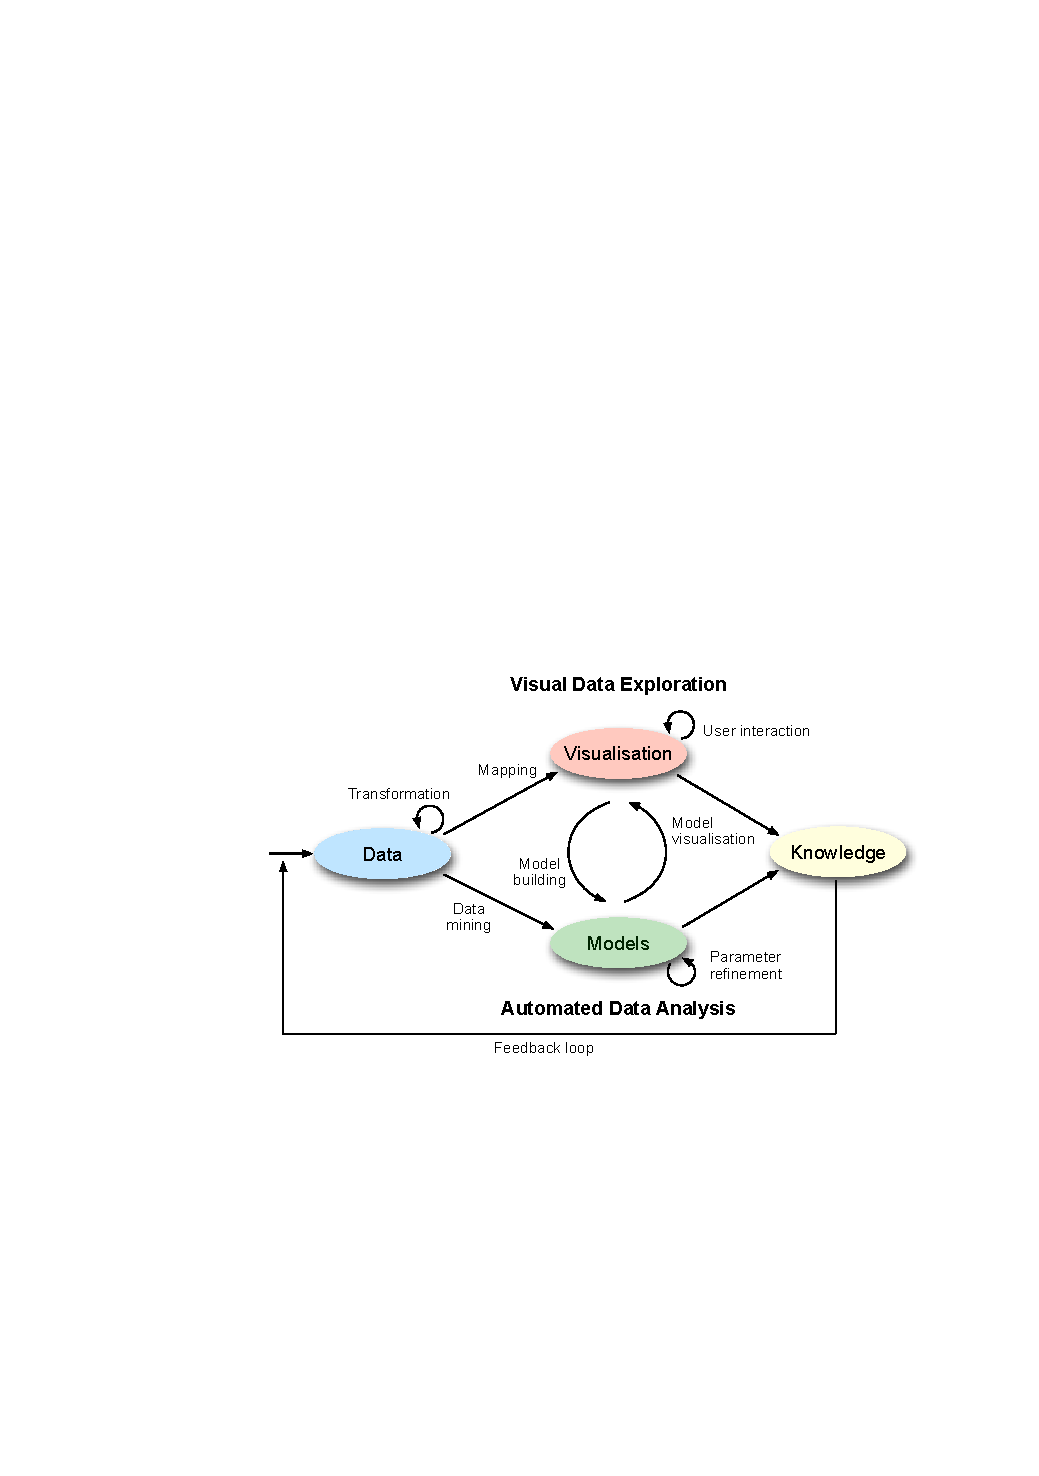
\includegraphics[width=\columnwidth]{visual-analytics-process}
%	\caption{The visual analytics process model. \emph{Source:~\cite{Keim2010}}.}
%	\label{fig:visual-analytics-process}
%\end{figure}
%
%
%Next, discuss basics of vis and models. and evaluation.

\subsection{Visualization Design}


\subsection{Automated Analysis Methods}
Data mining is the computational process of extracting patterns in large datasets~\cite{Tan2006}. Data mining tasks can be broadly divided into two major categories:

\begin{itemize}
		\item \emph{Descriptive tasks}. The objective is to derive patterns (correlations, trends, clusters, trajectories and anomalies) that summarizes the underlying relationships in data. Examples include cluster and association analyses. \emph{Clustering} aims to split data items to groups so that items within a group are more similar to each other than those in other groups. For example, clustering can be used to help marketers discover distinct groups of their customers before applying appropriate marketing strategies to those groups. \emph{Association} analysis discovers the connections among a set of data items. For example, it can be used to identify products that customers often purchase together such as bread and milk.
		
		\item \emph{Predictive tasks}. The objective is to predict the value of an unknown (target) attribute based on the values of other (explanatory) attributes. Examples include classification and regression. \emph{Classification} predicts discrete target variables whereas, \emph{regression} focuses on continuous ones. For example, predicting whether a customer buys a marketing product is a classification task because the target variable is binary. However, estimating a future house price is a regression task because price is a continuous-valued variable.
\end{itemize}

Next, we will discuss the clustering and classification tasks in more detail and how they are applied together with visualizations to help users gain deeper insight into the data. We also present some commonly used text mining techniques for exploring large sets of documents, which is essential in visual analytics~\cite{Thomas2005}.

\subsubsection{Clustering}

\paragraph{Overview}
Cluster analysis finds similarities between data points based on the characteristics of data attributes and groups similar data points into clusters. Clustering is regarded as \emph{unsupervised learning}~\cite{Han2011} because it can reveal hidden structure of a dataset that does not have \emph{labels} (or groups) defined. The most common clustering algorithm is \emph{k-means}~\cite{Lloyd1982}. Given a set of data points $(x_1, x_2, \dots, x_n)$, k-means clustering aims to partition them into $k$ clusters $(S_1, S_2, \dots, S_n)$, such that the within-cluster sum of squared distances is minimized: 
\[
\sum_{i=1}^k\sum_{x\in S_i} \lVert x-\mu_i \rVert^2
\]
where $\mu_i$ is the center of points (i.e., centroids) in $S_i$. 

The algorithms works as follows. Initially, partition data points into $k$ non-empty random subsets. Then, compute the centroids of the current clusters, and assign each data point to the cluster with the nearest centroid. Repeatedly recompute the centroids and reassign the cluster of each data point until no assignment can be done. This k-means clustering algorithm is efficient but often terminates at a local optimal. More detailed analysis of k-means and other clustering algorithms are out of the scope of this thesis and can be found in data mining textbooks~\cite{Tan2006,Han2011}.

\paragraph{Application Examples}
What is motion tracking data? What is the problem? What is clustered and how? How is a cluster visualized? What does the vis help?

Human motion tracking data has been applied in various research fields such as medicine, sports and animation~\cite{Bernard2013}. The data typically consists of temporal sequences of human poses represented by a set of 3D joint positions (e.g., head, hands, elbows and knees). However, analyzing a large collection of this temporal, high-dimensional dataset is challenging. To gaining an overall understanding of the data, MotionFlow~\cite{Jang2016} applies a k-means clustering method using a simple Euclidean distance of 3D joints as the similarity measurement. A cluster of human poses is represented as glyph with a stick figure showing the centroid of the cluster and semi-transparent ghosts around the center figure for other similar poses [todo figure 4]. MotionFlow uses a force-directed graph of clusters to illustrate their relationship with node distance mapping to the similarity of pose clusters and edges indicating the directed transition between two clusters. Edges are color coded to represent the transition frequency.

In MotionFlow, a user is allowed to interactively change the number $k$ of clusters, enabling exploration of the dataset. However, the re-clustering process may change all existing clusters and make it difficult for the user to keep track. To address this issue, MotionFlow allows the user to select the clusters to be locked or unchanged during the re-clustering process. He or she is also able to interactively merge or split clusters according to her or his own assessment.

To achieve the same objective of gaining an overall understanding of human motion tracking data, MotionExplorer~\cite{Bernard2013} applies a different cluster analysis method -- hierarchical clustering~\cite{Han2011} -- which seeks to build a hierarchy of clusters. MotionExplorer takes a decisive approach considering all data items initially are in the same cluster and splitting them until a termination condition is met. One of the important decisions in this clustering technique is to determine which cluster to split next. The user is allowed to choose among several splitting strategies such as the maximum standard deviation to split the most varied cluster first and the highest number of elements to split the largest cluster first. The hierarchy 
A clustering of the data objects is obtained by cutting
the dendrogram at the desired level, then each
connected component forms a cluster
hierarchical clustering: MotionExplorer
spatial+temporal clustering: MobilityGraph 
aggolemeative clustering: NewsLab
BiSet: biclustering
without clustering algorithm: force layout with correlation

\subsubsection{Classification}
Classification predicts the value of a categorical (discrete or nominal) attribute based on the values of other attributes. It builds a model (or \emph{classifier}) based on a labeled training dataset (i.e., \emph{supervised learning}) and applies it in labeling new data~\cite{Han2011}. The model needs to not only identify the labels in the training dataset well but also be general enough to predict the labels of new data correctly. One common and intuitive classification algorithm is decision tree induction~\cite{Quinlan1986}. Each non-leaf node represents a ``test'' on an attribute, which splits the node to multiple branches, each for an outcome of the test. Each leaf node is associated with a class label and is the result of a sequence of tests starting from the root node.

The importance of building a decision tree is choosing which attribute to split at each node. Intuitively, we should choose attributes that can divide nodes into ``pure'' child nodes so that all data items in a child node belong to a single class and no further splits is needed. For example, in a binary classification, consider a training dataset with 10 records, 5 labeled ``true'' and 5 labeled ``false''. Attribute $A1$ splits the set to two subsets: (5 ``true'', 0 ``false'') and (0 ``true'', 5 ``false''). Attribute $A2$ splits the set to (3 ``true'', 2 ``false'') and (2 ``true'', 3 ``false''). The subsets split by $A1$ is ``purer'' than the one by $A2$ because they do not contain a mix of ``true'' and ``false''. To achieve this purity, several attribute measurements have been proposed such as \emph{information gain} and \emph{gini index}~\cite{Tan2006}. More detailed analysis of these measurements and other classification algorithms are out of the scope of this thesis and can be found in data mining textbooks~\cite{Tan2006,Han2011}.

TODO: more specific classification techniques/applications and how vis helps improve understanding

\subsubsection{Information Design Principles}
\label{sub:lr-design}

\paragraph{Marks and Channels}
Marks are basic geometric elements that depict items or links, and channels control their appearance~\cite{Munzner2014}. Item marks can be zero-dimensional as a \emph{point}, one-dimensional as a \emph{line}, two-dimensional as an \emph{area}, and three-dimensional as a \emph{volume}, but rarely used. Link marks include \emph{connection} showing a pairwise relationship between two items using a line and \emph{containment} showing hierarchical relationships using areas. \autoref{fig:lr-marks} illustrates these marks. 

\begin{figure}[!htb]
	\centering
	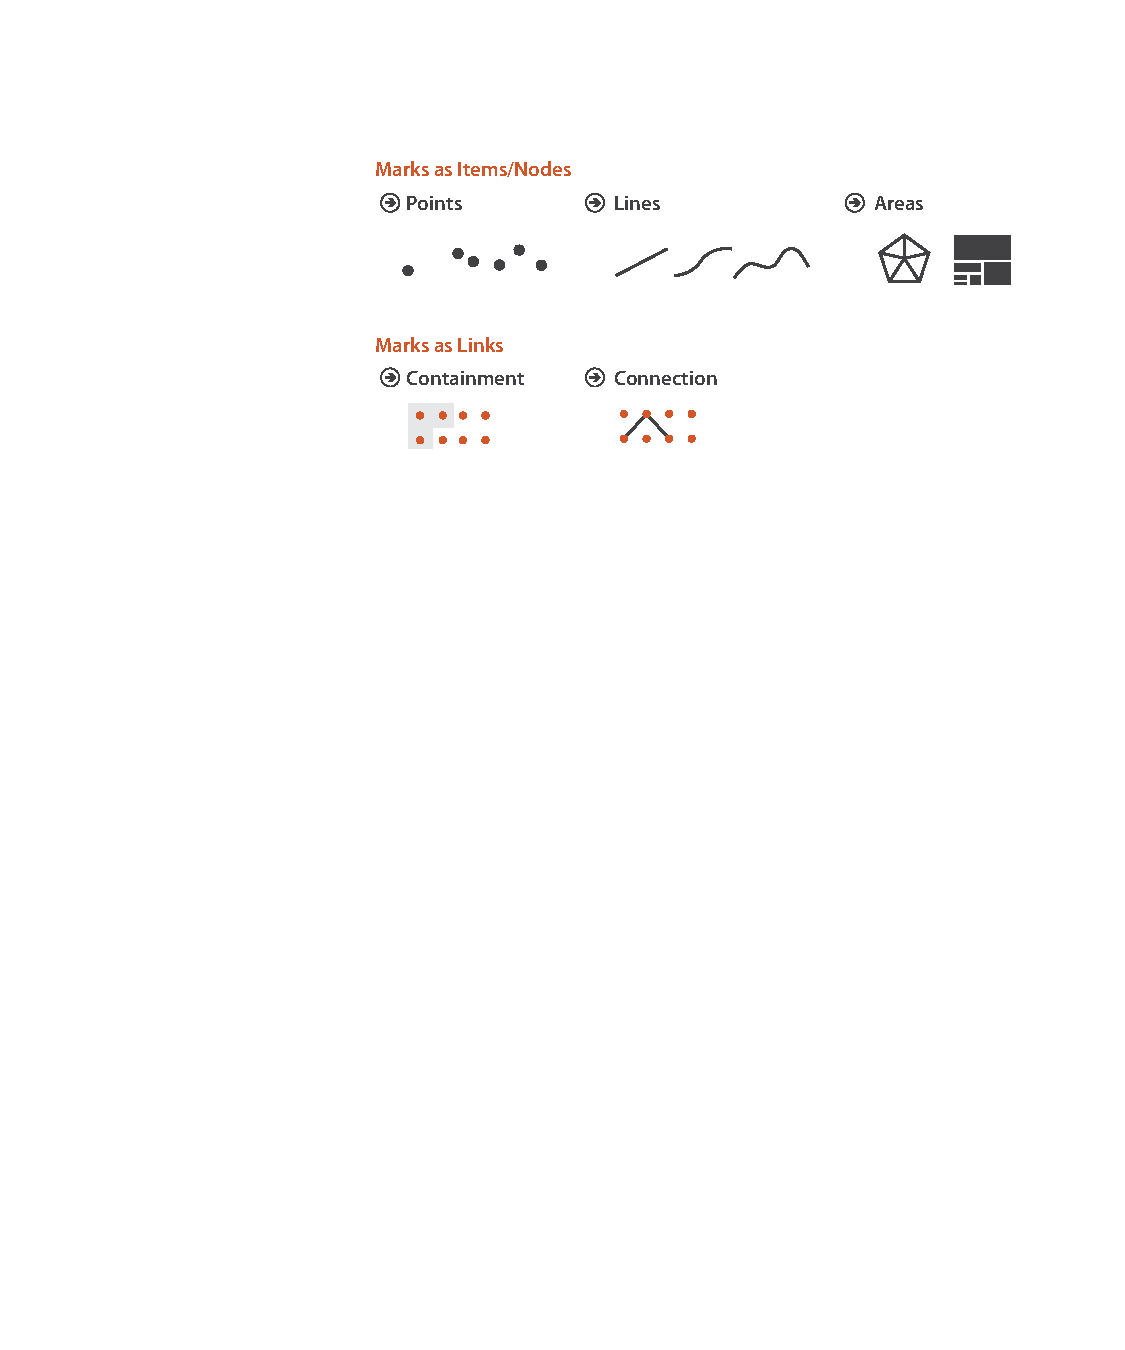
\includegraphics[width=.8\linewidth]{marks}
	\caption{Item and link marks as geometric primitives. \is{Munzner2014}}
	\label{fig:lr-marks}
\end{figure}

A visual channel control the appearance of marks, independent of their dimensionality. Examples include position, color, shape, angle and size. However, not all channels can be applied to all marks. For instance, an area mark is used in a geographic map to denote a region. It is already associated with a shape and size, thus cannot be size coded to represent another quantitative attribute.
some visual channels. some cannot encode size, example. \autoref{fig:lr-channel-example} shows a progression of chart types, with each showing one more data attribute using one more visual channel. \autoref{fig:lr-channel-example-1} shows a bar chart representing a single quantitative attribute using the \emph{vertical position} channel. \autoref{fig:lr-channel-example-2} shows a scatter plot encoding the second quantitative attribute using the \emph{horizontal position} channel. \autoref{fig:lr-channel-example-3} adds the \emph{color} channel to represent a categorical attribute, and \autoref{fig:lr-channel-example-4} adds the \emph{size} channel to represent another quantitative attribute. In these examples, each attribute is encoded with a single channel. However, multiple channels can be combined to redundantly encode the same attribute, helping perceive it more easily.

\begin{figure}[!htb]
\centering
\subcaptionbox{Line marks with horizontal position for a categorical attribute and vertical position for a quantitative attribute.\label{fig:lr-channel-example-1}}{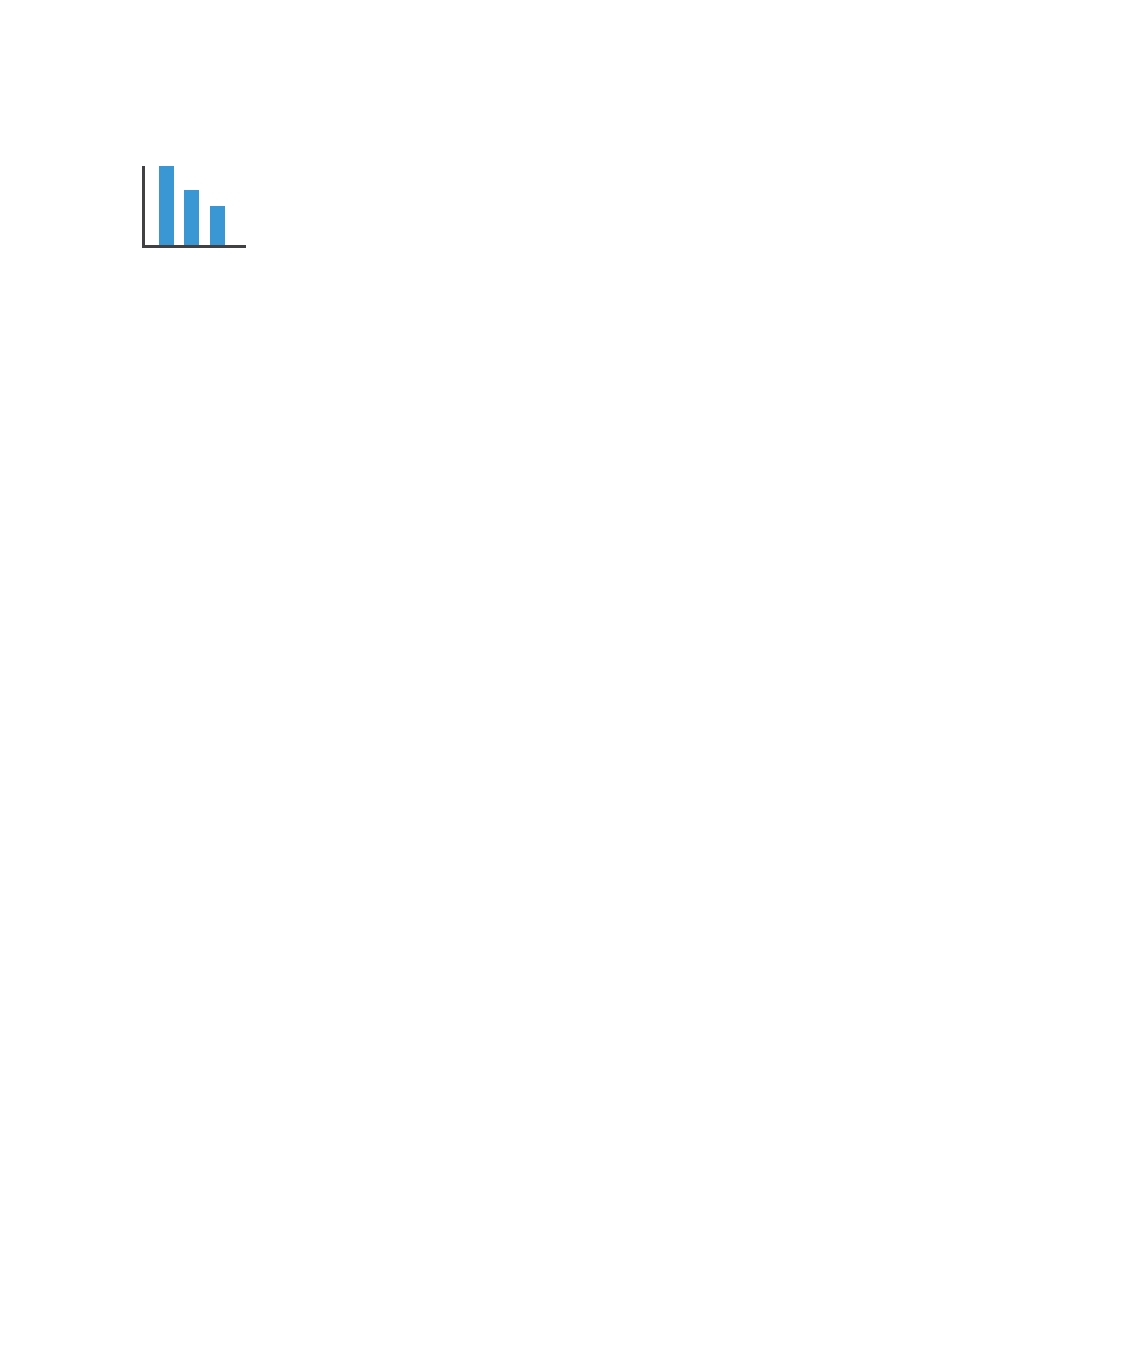
\includegraphics[width=.23\columnwidth]{channel-example-1}} 
\hfill
\subcaptionbox{Point marks with both horizontal and vertical position channels for quantitative attributes.\label{fig:lr-channel-example-2}}{
\includegraphics[width=.23\columnwidth]{channel-example-2}} 
\hfill
\subcaptionbox{A categorical attribute is added using the color channel.\label{fig:lr-channel-example-3}}{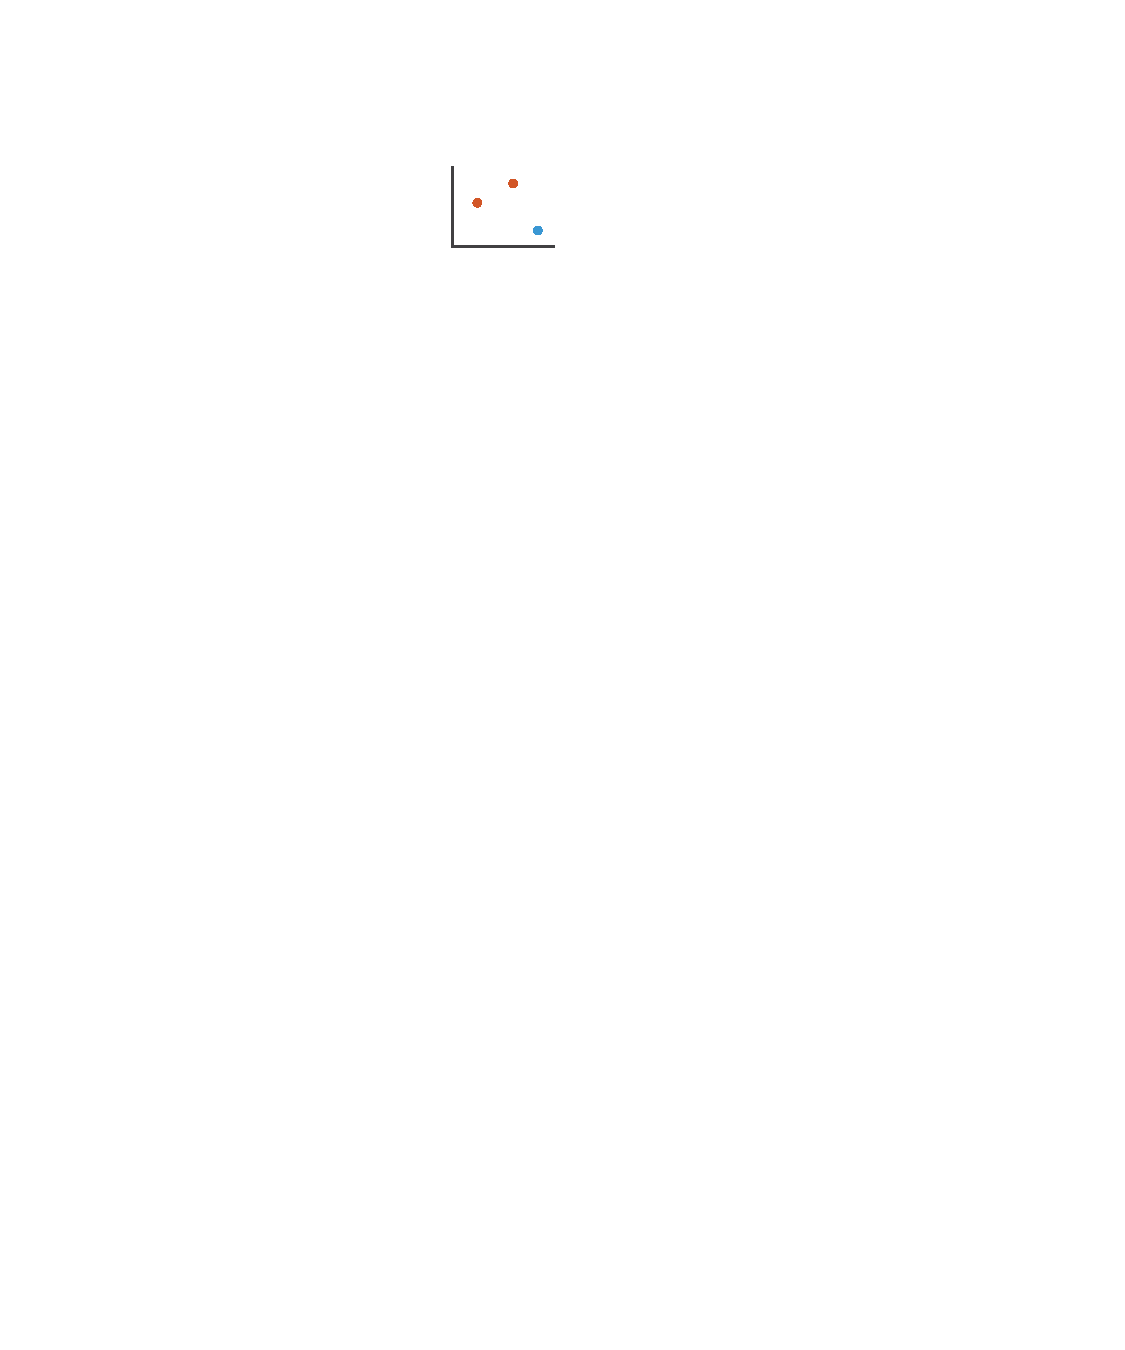
\includegraphics[width=.23\columnwidth]{channel-example-3}}
\hfill
\subcaptionbox{Another quantitative attribute is added using the size channel.\label{fig:lr-channel-example-4}}{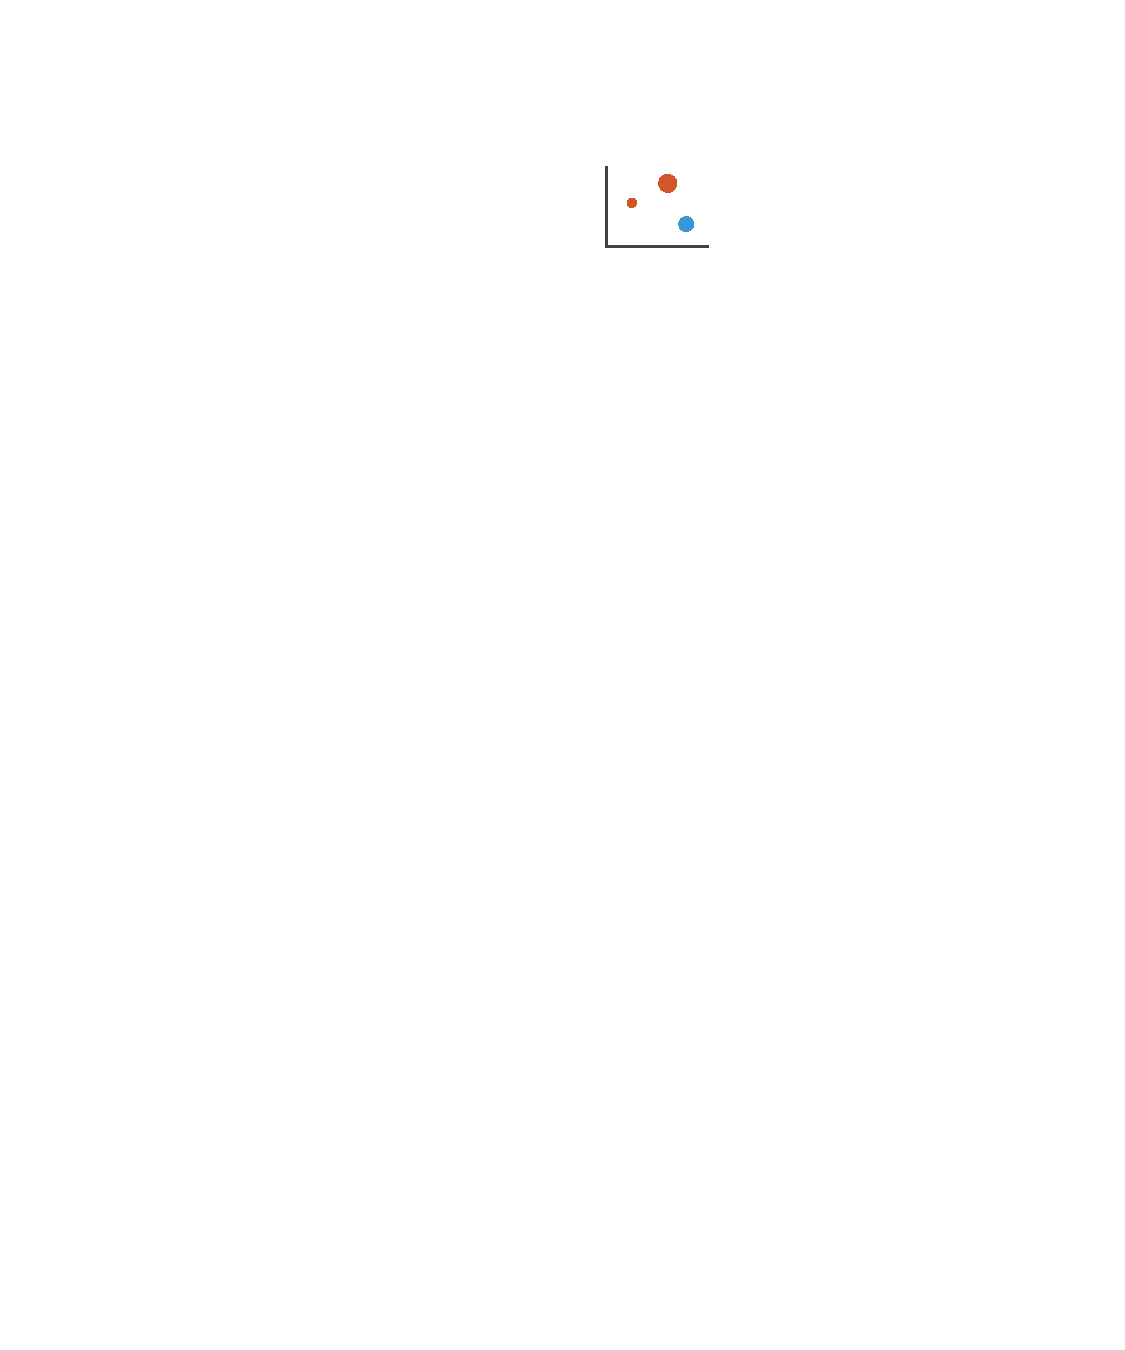
\includegraphics[width=.23\columnwidth]{channel-example-4}}
\caption{Using marks and channels.}
\label{fig:lr-channel-example}
\end{figure}

All channels are not equal; they are processed and perceived differently by our human visual systems. Also, not all channels are appropriate for encoding both ordered and categorical attributes. Ordered attributes should be shown using magnitude channels, with \emph{aligned spatial position} as the most effective channel and \emph{3D volume} as the least effective one. Categorical attributes should be shown using identity channels, with \emph{spatial region} as the most effective channel and \emph{shape} as the least effective one. \autoref{fig:lr-channel-ranking} shows the detailed ranking of effectiveness of many visual channels, separated by the type of attribute. This ranking is documented by Munzner~\cite{Munzner2014}, based on many empirical studies such as the work by Cleveland and McGill~\cite{Cleveland1985}, and by Heer and Bostock~\cite{Heer2010a}.

\begin{figure}[!htb]
	\centering
	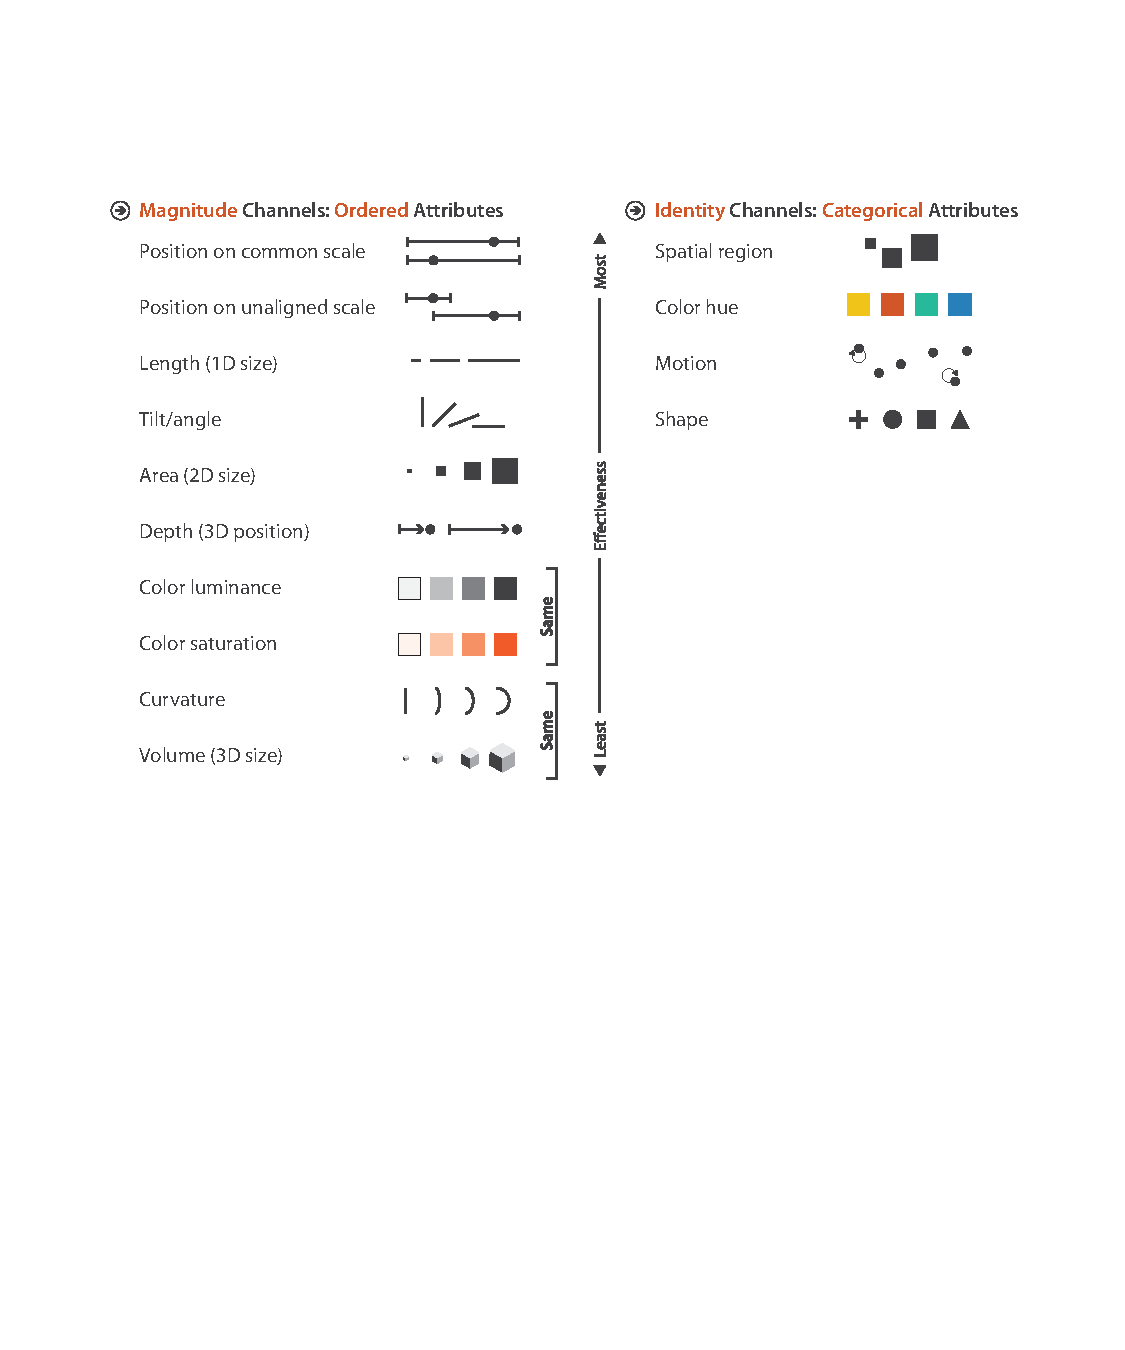
\includegraphics[width=\linewidth]{channel-ranking}
	\caption{Channels ranked by effectiveness according to data and channel type. \is{Munzner2014}}
	\label{fig:lr-channel-ranking}
\end{figure}

Color is a special channel that can be used for both data attributes. As shown in \autoref{fig:lr-channel-ranking}, color luminance and saturation are used in magnitude channels, and color hue is used in identity channels. A colormap specifies a mapping between colors and data values, and designing an effective colormap is challenging. ColorBrewer~\cite{Harrower2003} is an excellent source for colormap reference, providing color schemes for both categorical and ordered attributes. Human can only distinguish around 12 colors simultaneously~\cite{Munzner2014}. \autoref{fig:lr-colorbrewer-1} shows such a categorical colormap with 12 distinguished color hues. Ordered colormaps can be either sequential (\autoref{fig:lr-colorbrewer-2}) or diverging (\autoref{fig:lr-colorbrewer-3}). Diverging colormaps use two different color hues to emphasize values below and above the middle point.

\begin{figure}[!htb]
\centering
\subcaptionbox{Categorical colormap with distinguishable color hues.\label{fig:lr-colorbrewer-1}}[\columnwidth]{
\includegraphics[width=.6\columnwidth]{colorbrewer-1}} 
\\
\subcaptionbox{Sequential colormap: a single color hue with different saturation level.\label{fig:lr-colorbrewer-2}}[\columnwidth]{\hspace{-.15\columnwidth}
\includegraphics[width=.45\columnwidth]{colorbrewer-2}}
\\
\subcaptionbox{Diverging colormap: two color hues emphasizing positive and negative values.\label{fig:lr-colorbrewer-3}}[\columnwidth]{\hspace{-.05\columnwidth} 
\includegraphics[width=.55\columnwidth]{colorbrewer-3}}
\caption{Colormaps from ColorBrewer. \is{Harrower2003}}
\end{figure}

\subparagraph{Gestalt Principles}
\label{sub:lr-gestalt}
Gestalt principles describe how we see patterns in visual displays~\cite{Koffka1935}. This section reviews three commonly used principles in representing groups of items.

\subparagraph{Similarity} 
Similar elements tend to be grouped together. \autoref{fig:lr-gestalt-similarity-1} shows a matrix of point marks with uniform spacing, but using two different shapes: dot and cross. The similarity of shapes helps us see the rows more clearly than the columns. Two separable channels can be applied together to reveal patterns by either rows or columns. In \autoref{fig:lr-gestalt-similarity-2}, green is used to depict rows, and texture is used to depict columns.

\begin{figure}[!htb]
\centering
\subcaptionbox{Similarity of shapes distinguishes rows.\label{fig:lr-gestalt-similarity-1}}[.47\columnwidth]{
\includegraphics[height=.35\columnwidth]{gestalt-similarity-1}} 
\hfill
\subcaptionbox{Color and texture delineate rows and columns, respectively.\label{fig:lr-gestalt-similarity-2}}[.47\columnwidth]{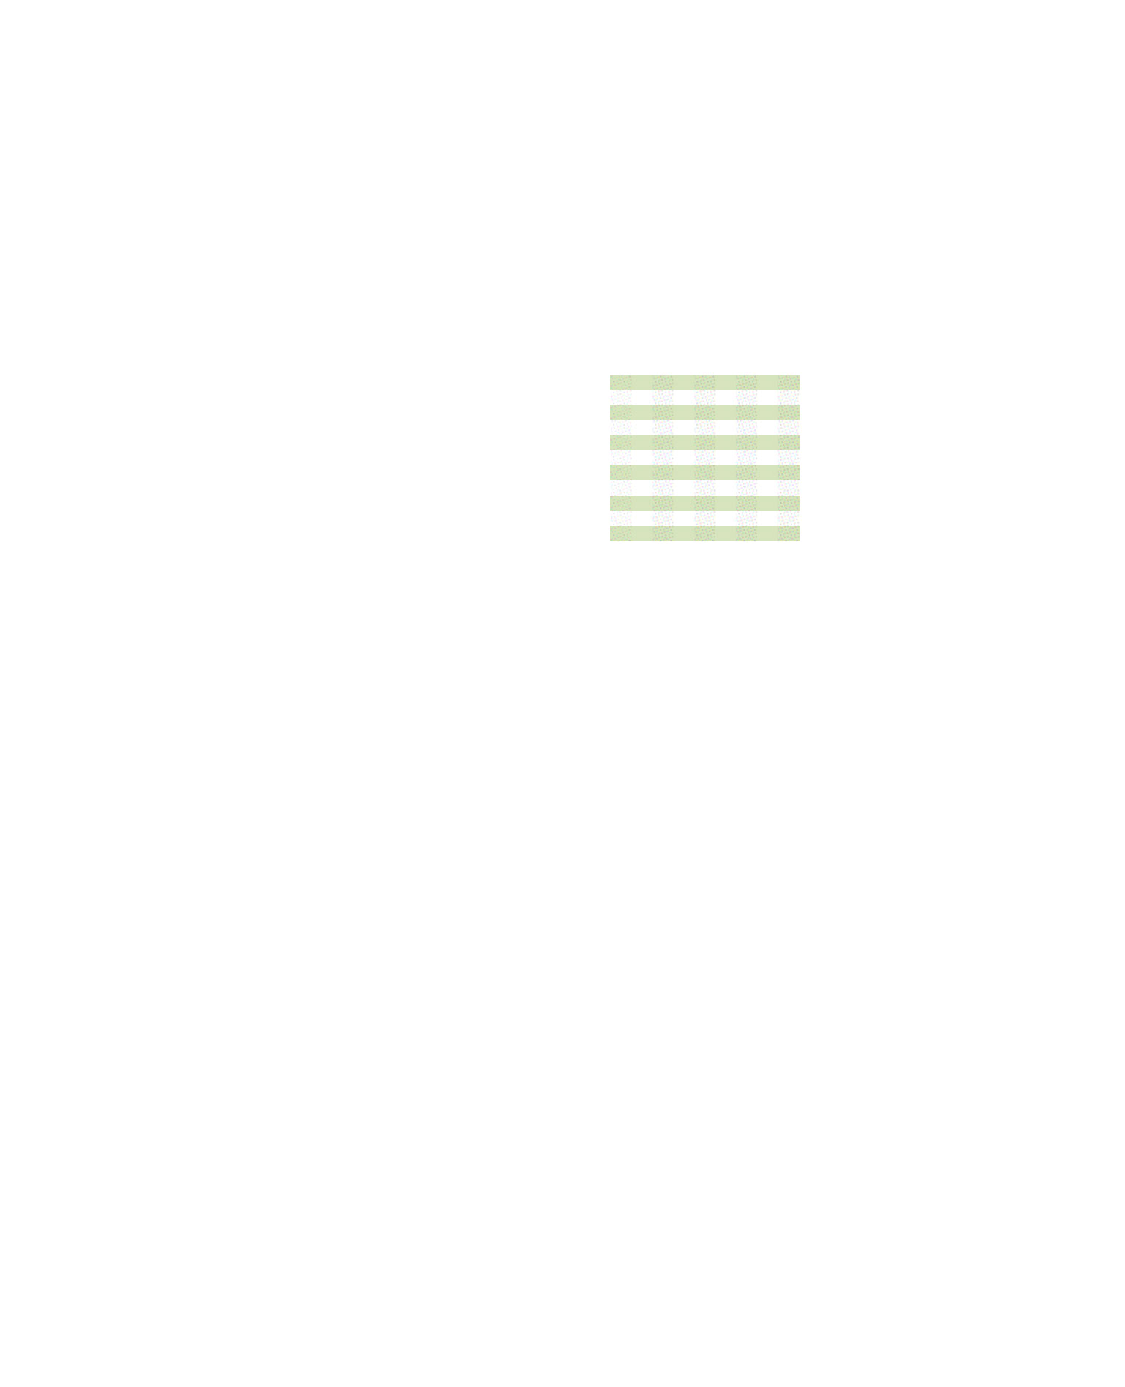
\includegraphics[height=.35\columnwidth]{gestalt-similarity-2}} \label{fig:lr-gestalt-similarity}
\caption{Similarity principle: similar elements are perceived as a group. \is{Ware2013}}
\end{figure}

\subparagraph{Proximity} 
Elements that are close together are perceptually grouped together. \autoref{fig:lr-gestalt-proximity-1} clearly shows two groups of dots. \autoref{fig:lr-gestalt-proximity-2} shows rows of dots. However, with a small change of spacing, these dots are perceived as columns in \autoref{fig:lr-gestalt-proximity-3}. The application of this principle is straightforward: organizing related information close together. It helps separate groups of unrelated objects and facilitates searching for information.

\begin{figure}[!htb]
\centering
\subcaptionbox{Two groups of dots.\label{fig:lr-gestalt-proximity-1}}{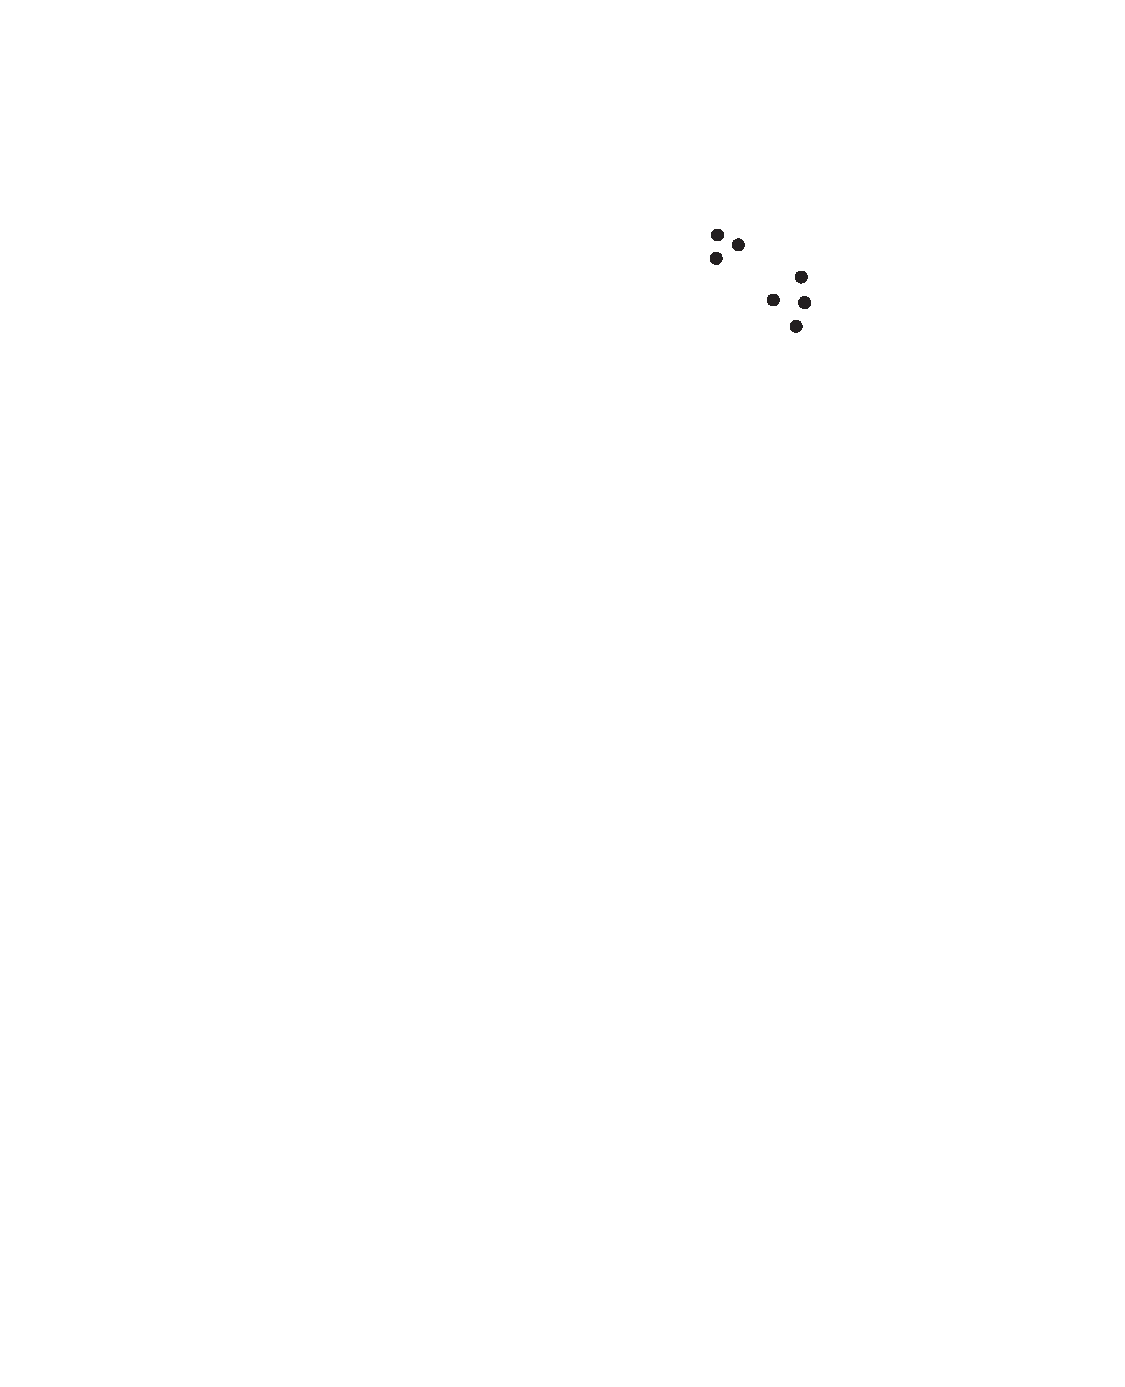
\includegraphics[width=.25\columnwidth]{gestalt-proximity-1}} 
\hfill
\subcaptionbox{Rows of dots.\label{fig:lr-gestalt-proximity-2}}{
\includegraphics[width=.31\columnwidth]{gestalt-proximity-2}} 
\hfill
\subcaptionbox{Columns of dots.\label{fig:lr-gestalt-proximity-3}}{
\includegraphics[width=.31\columnwidth]{gestalt-proximity-3}}
\label{fig:lr-gestalt-proximity}
\caption{Spatial proximity principle: spatially close elements are perceived as a group. \is{Ware2013}}
\end{figure}

\paragraph{Connectedness} 
Elements that are connected by visual properties are perceived as being more related than elements that are not connected. This principle can be achieved simply by drawing a border around a group of elements as in \autoref{fig:lr-gestalt-connectedness-1}. This is extensively applied in designing complex graphical user interface: groups of related features are separated by borders. Another approach to implement connectedness is by drawing lines between related elements as in \autoref{fig:lr-gestalt-connectedness-2}. This is the basics of \emph{node-link diagrams} -- one of the most common methods of representing relationships between elements.

\begin{figure}[!htb]
\centering
\subcaptionbox{Using border to denote a group.\label{fig:lr-gestalt-connectedness-1}}{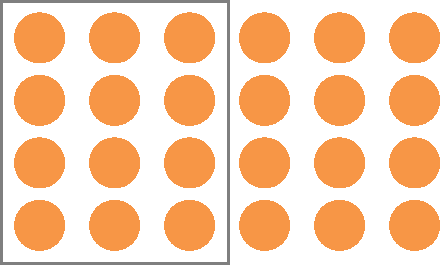
\includegraphics[width=.4\columnwidth]{gestalt-connectedness-1}} 
\hfill
\subcaptionbox{Using lines to denote a group.\label{fig:lr-gestalt-connectedness-2}}{
\includegraphics[width=.4\columnwidth]{gestalt-connectedness-2}} 
\caption{Connectedness principle: visually connected elements are perceived as a group. \is{Ware2013}}
\label{fig:lr-gestalt-connectedness}
\end{figure}

Among these three Gestalt principles of representing groups of elements, connectedness has the strongest effect, followed by proximity and then similarity. \autoref{fig:lr-gestalt} illustrates this comparison. In \autoref{fig:lr-gestalt-1}, even though spacing between dots in rows is shorter than spacing between dots in columns, the lines make the vertical links clearer than rows. In \autoref{fig:lr-gestalt-2}, the lines also make the horizontal links more notable than groups of colored circles. In \autoref{fig:lr-gestalt-3}, two spatial groups are more clearly perceived than colored groups.

\begin{figure}[!htb]
\centering
\subcaptionbox{Links are more clearly perceived than spatial groups.\label{fig:lr-gestalt-1}}[.3\columnwidth]{
\includegraphics[height=.12\columnwidth]{gestalt-1}} 
\hfill
\subcaptionbox{Links are more clearly perceived than colored groups.\label{fig:lr-gestalt-2}}[.3\columnwidth]{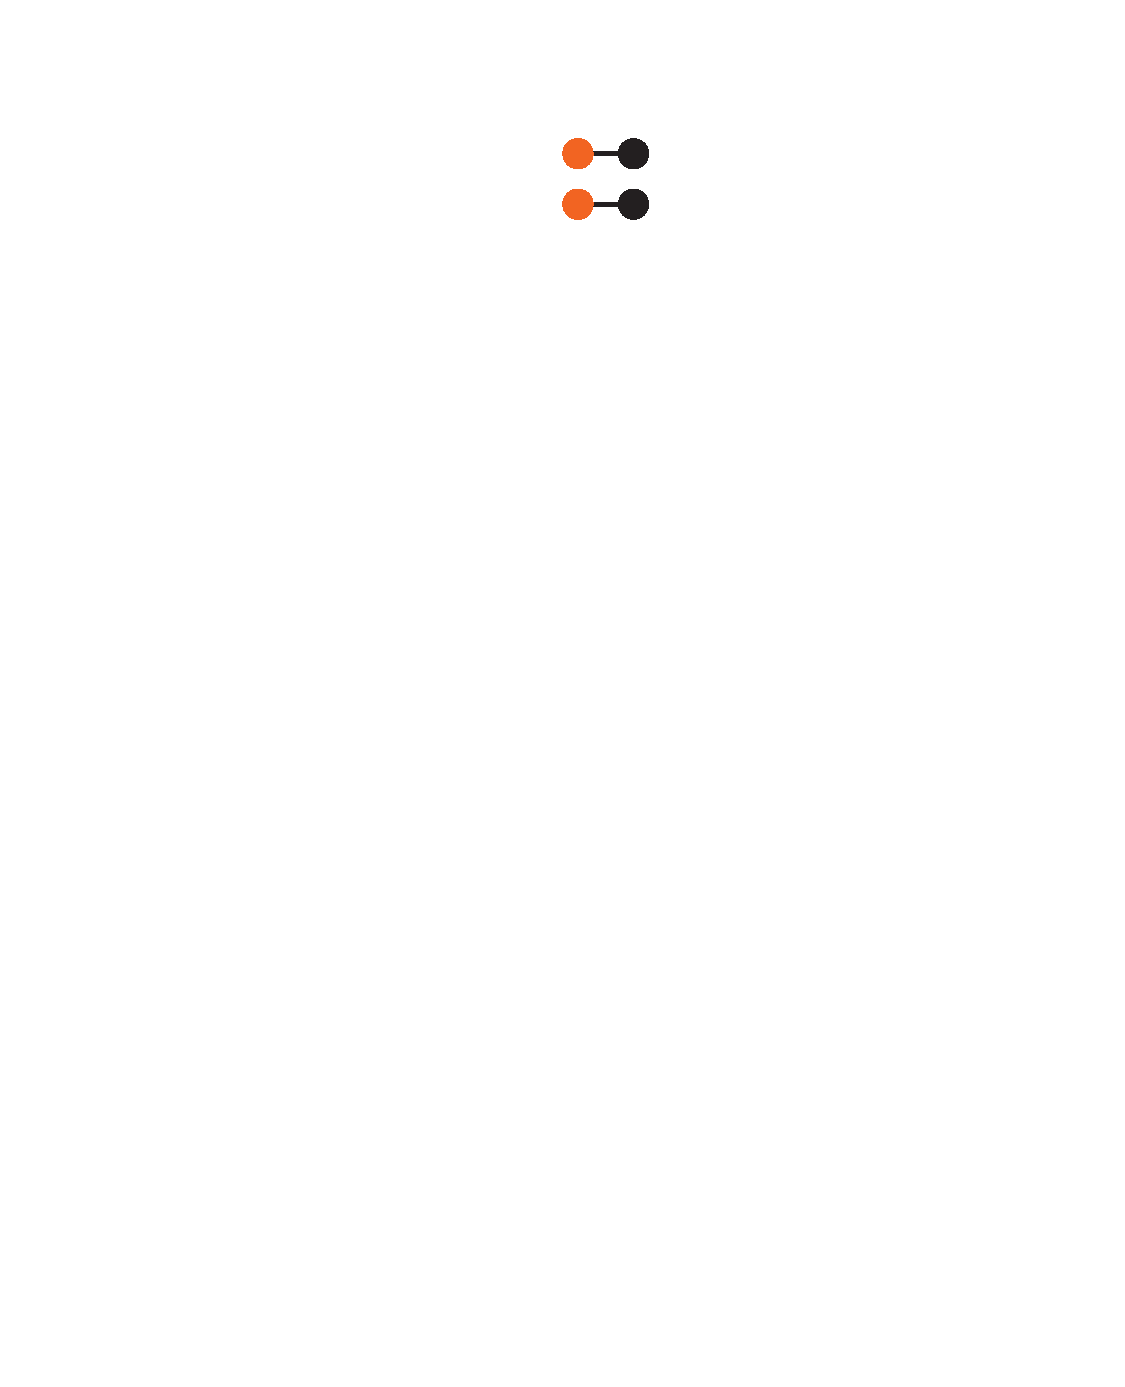
\includegraphics[height=.12\columnwidth]{gestalt-2}} 
\hfill
\subcaptionbox{Spatial groups are more clearly perceived than colored groups.\label{fig:lr-gestalt-3}}[.3\columnwidth]{
\includegraphics[height=.12\columnwidth]{gestalt-3}}
\caption{Comparison of Gestalt principles. Connectedness is stronger than proximity, and proximity is stronger than similarity. \is{Ware2013}}
\label{fig:lr-gestalt}
\end{figure}

\paragraph{Tufte's Principles}
Tufte proposes a number of principles for a well-designed graphic, documented in his series of books, most notably including \emph{The Visual Display of Quantitative Information}~\cite{Tufte1983} and \emph{Envisioning Information}~\cite{Tufte1990}. This section reviews a few principles that have been commonly applied in graphic design and visualization.

\subparagraph{Graphical Integrity}
This principle emphasizes that the graphical representation should tell the truth about the data. Representation of numbers, as physically measured on the surface of the	graphic	itself,	must be directly proportional to the numerical quantities represented~\cite{Tufte1983}. \autoref{fig:lr-tufte-integrity-1} shows a falsely big drop in stock market value between 2001 and 2002. It because the chart uses a relative scale with the value range from 450 to 500, causing its height disproportional to the market value. \autoref{fig:lr-tufte-integrity-2} corrects this error by using an absolute scale with the value range starting from 0.

\begin{figure}[!htb]
\centering
\subcaptionbox{Using a relative value range causes a falsely big drop of stock market value between 2001 and 2002.\label{fig:lr-tufte-integrity-1}}{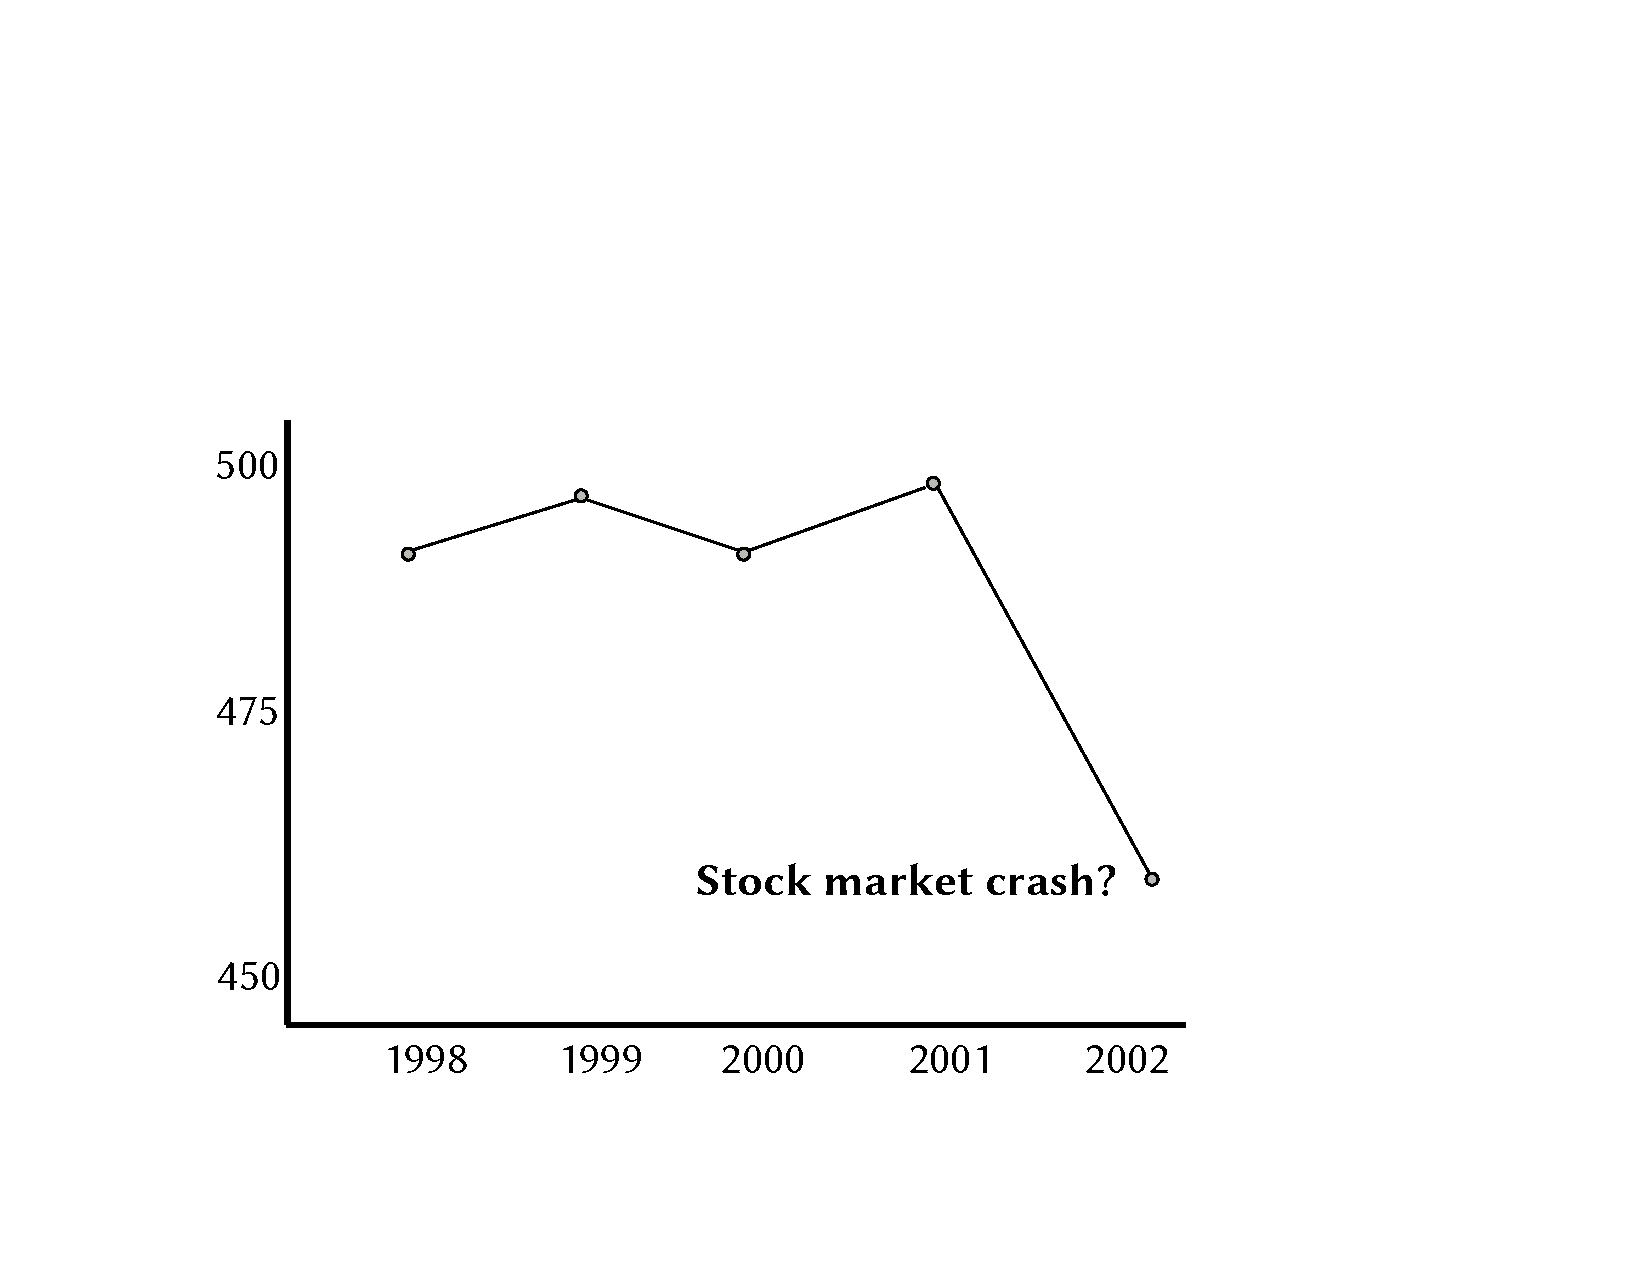
\includegraphics[width=.47\columnwidth]{tufte-integrity-1}} 
\hfill
\subcaptionbox{Using an absolute value range to depict the data accurately.\label{fig:lr-tufte-integrity-2}}{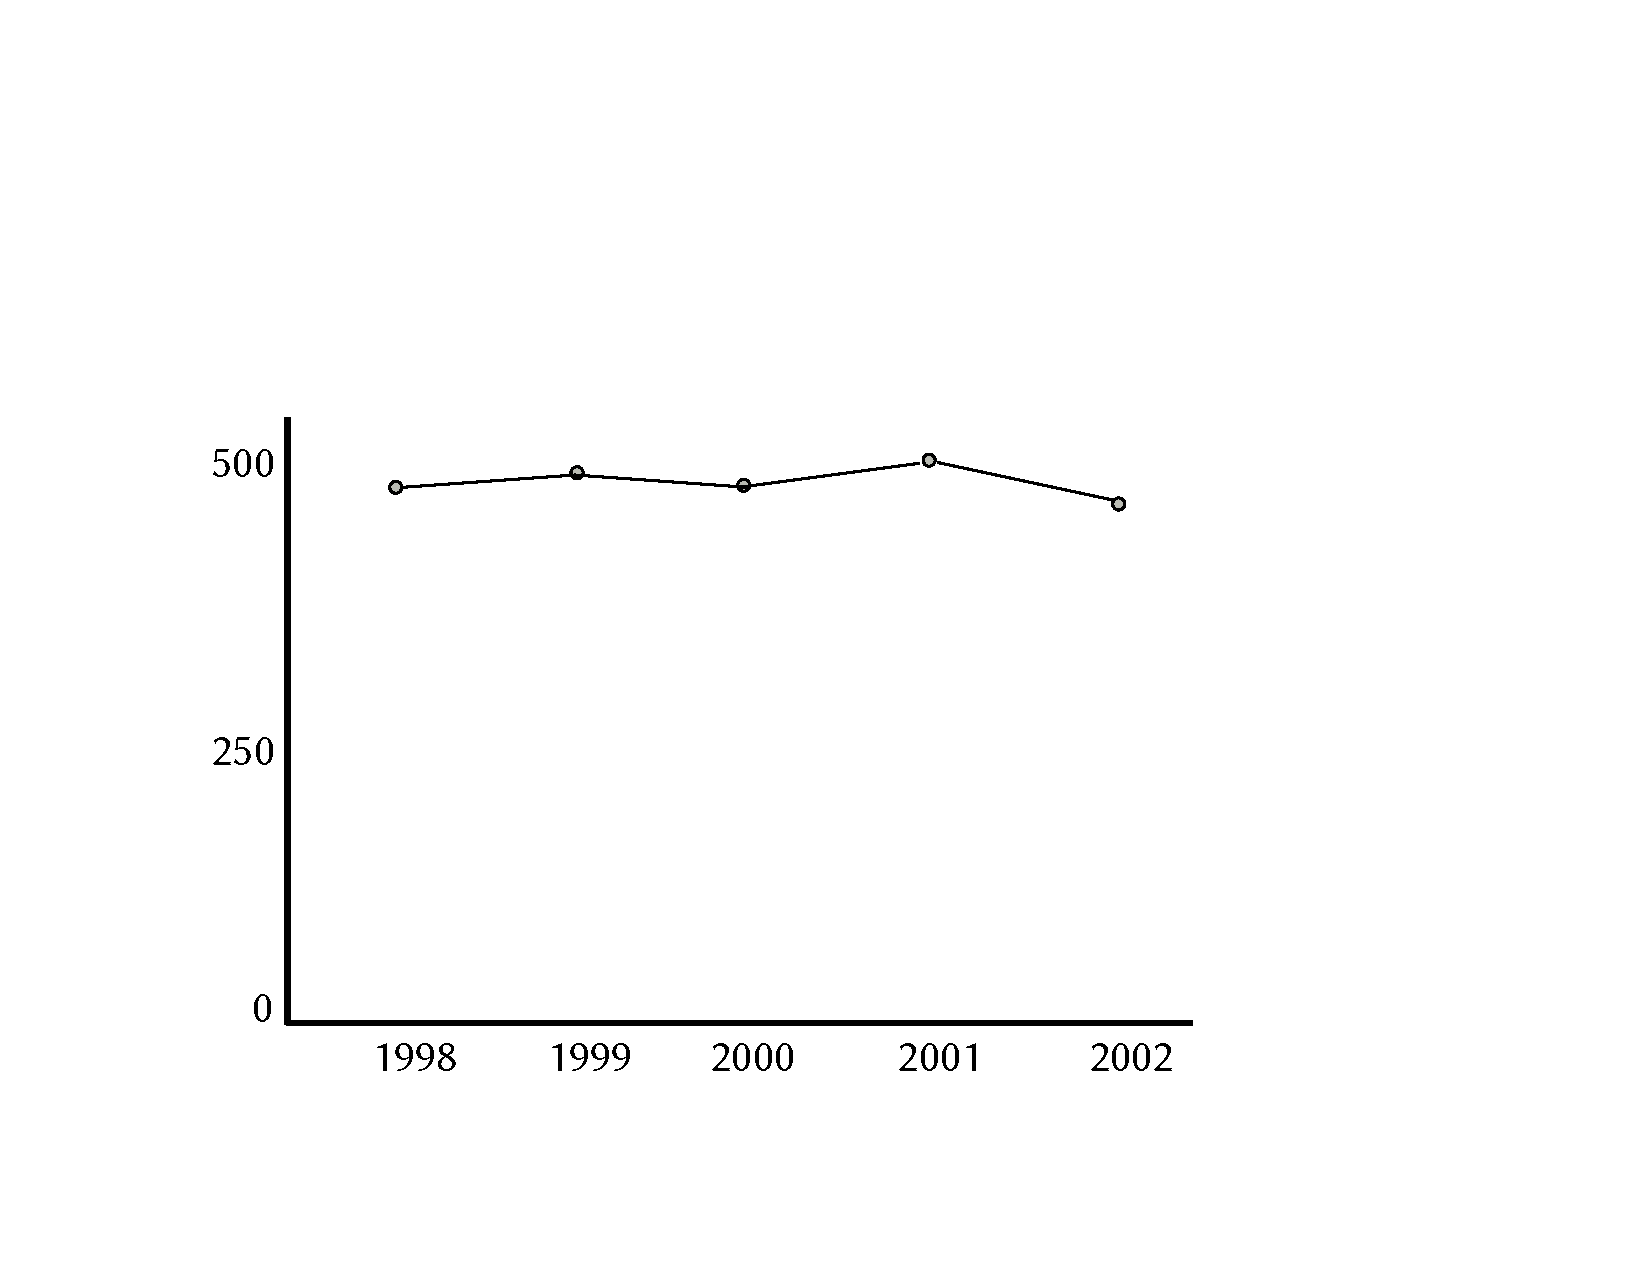
\includegraphics[width=.47\columnwidth]{tufte-integrity-2}} 
\caption{Graphical integrity principle. The chart should tell the truth about the data.}
\label{fig:lr-tufte-integrity}
\end{figure}

\subparagraph{Data-Ink Ratio Maximization}
Data-ink includes the pixels in the graphic that are used for representing the data. Data-ink ratio is defined as the ratio between the data-ink and the total non-background pixels used in the graphic. This principle aims to maximize this ratio by erasing non-data-ink and erasing redundant data-ink.

\begin{figure}[!htb]
\centering
\subcaptionbox{A bar chart with poor data-ink ratio.\label{fig:lr-tufte-ink-1}}{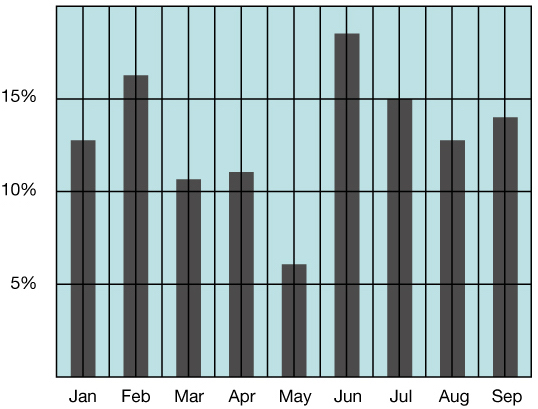
\includegraphics[width=.47\columnwidth]{tufte-ink-1}} 
\hfill
\subcaptionbox{A bar chart with high data-ink ratio by removing background, border and grid lines.\label{fig:lr-tufte-ink-2}}{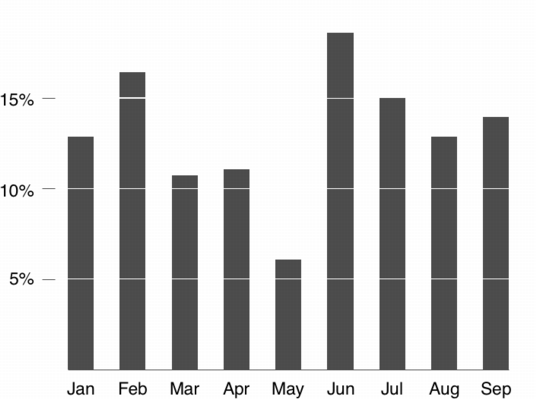
\includegraphics[width=.47\columnwidth]{tufte-ink-2}} 
\caption{Data-ink ratio maximization principle: removing the graphic that does not contribute to the understanding of the data.}
\label{fig:lr-tufte-ink}
\end{figure}
% Source: http://www.infovis-wiki.net/index.php/Data-Ink_Ratio

\subparagraph{Micro/Macro Readings}
This principle suggests that a graphic can contain both enormous details and an overall pattern. This allows the viewer to glance from a distance to observe the big picture, and later drill-down closely to examine its individual pieces. Classic stem-and-leaf plot is a great example to illustrate this principle (\autoref{fig:lr-tufte-micro}). The plot shows all individual data items at meaningful level of detail, and provides an understanding of the data distribution. The micro/macro principle is extensively applied in interactive visualization, where zooming are panning are made possible, such as Google Maps. Data items at different scales can be represented with different levels of detail to provide appropriate information based on the allowed display area.

\begin{figure}[!htb]
	\centering
	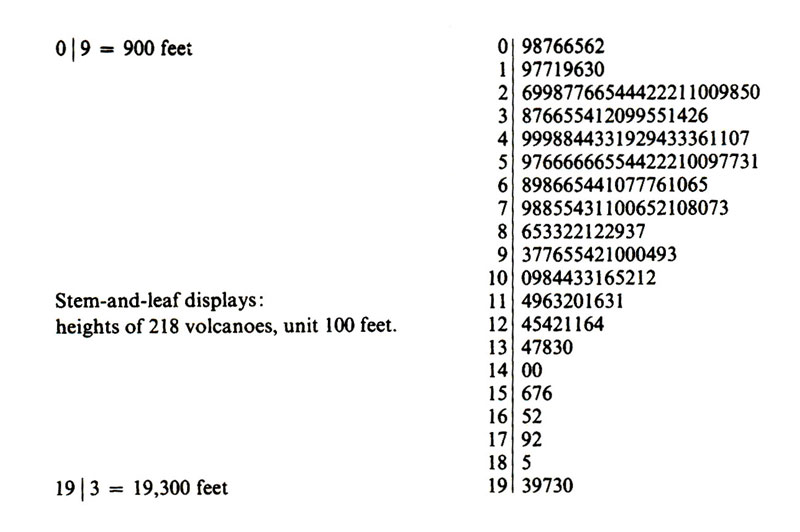
\includegraphics[width=.9\linewidth]{tufte-micro}
	\caption{Micro/macro principle. A stem-and-leaf plot shows both the data distribution and individual items. \is{Tufte1983}}
	\label{fig:lr-tufte-micro}
\end{figure}


%In a broader context, GUI design principles:  Schneiderman~\cite{Shneiderman2016} (eight golden rules), Norman (six design principles) ~\cite{Norman2002} and	Nielsen (ten usability heuristics)~\cite{Nielsen1994} -- create a table with rows showing similar principles
%http://www.csun.edu/science/courses/671/bibliography/preece.html
%https://faculty.washington.edu/jtenenbg/courses/360/f04/sessions/schneidermanGoldenRules.html
%https://www.interaction-design.org/literature/article/shneiderman-s-eight-golden-rules-will-help-you-design-better-interfaces

\subsubsection{Interaction Techniques}
Interaction typically refers to the set of controls provided to the user to manipulate an interface~\cite{Pike2009a}. A static visualization may only show one aspect of a dataset. When the dataset is large enough, showing all the data at once may also make the visualization become cluttered. Interaction plays an important role in solving these problems. It can help explore large datasets at multiple levels of detail, identify patterns through examination of different visual representations and understand the connections between them.

Examples of interaction include standard techniques used in graphical user interface such as mouse clicking and scrolling, and more visualization specific techniques such as \emph{linking and brushing}~\cite{Kosara2003}, and \emph{focus+context}~\cite{Cockburn2008}. Multiple views in a visualization are often linked together to exploit their strengths. The user can select points of interest using the brushing technique, typically done directly on the visual data representation such as dragging a rectangular area. The points are brushed in one view will be highlighted in other views, allowing the user to explore them with different perspectives and representations (\autoref{fig:lr-linking}). Focus+Context is a technique that brings both the overview (context) and the detailed information (focus) together in one view. A fisheye view~\cite{Furnas1986,Furnas2006} is one example of this technique: the focal region is magnified and displayed within its surrounding context (\autoref{fig:lr-fisheye}).

\begin{figure}[!htb]
\centering
\subcaptionbox{Linking and brushing. Data points brushed in one view are linked and highlighted in other views.\label{fig:lr-linking}}{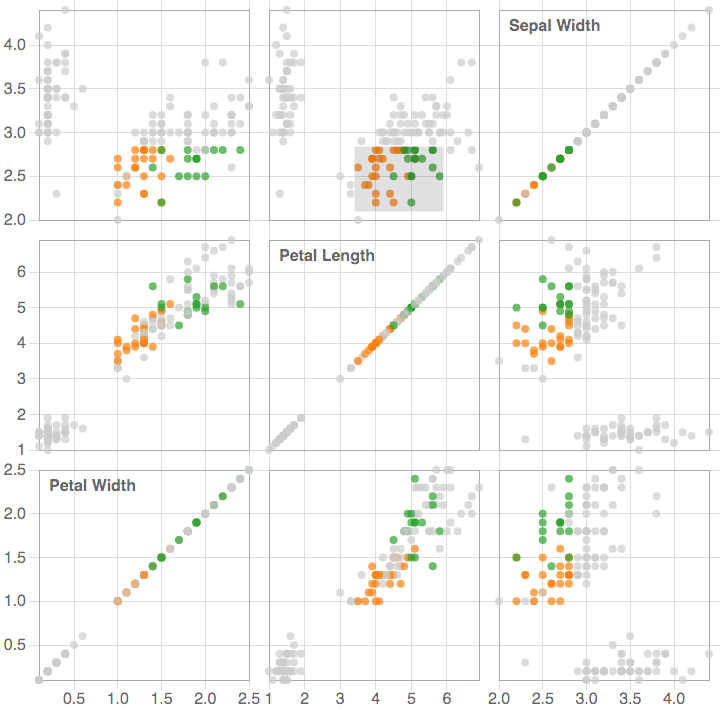
\includegraphics[height=.43\columnwidth]{linking}} 
\hfill
\subcaptionbox{Fisheye view for focus+context. Both the overview and the detailed information are displayed in one view.\label{fig:lr-fisheye}}{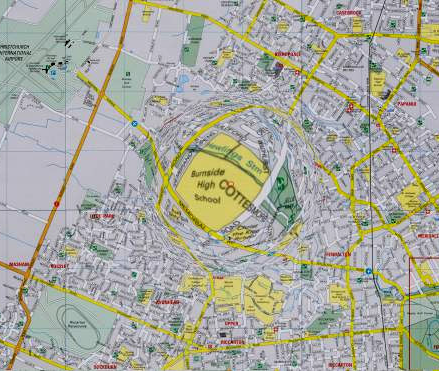
\includegraphics[height=.43\columnwidth]{fisheye}} 
\caption{Examples of interaction techniques.}
\label{fig:lr-interaction}
\end{figure}

Many other interaction techniques can be found in the taxonomies by Dix and Ellis~\cite{Dix1998}, by Keim~\cite{Keim2002}, and by Wilkinson~\cite{Wilkinson2005}. Very often, a user performs an interaction to achieve some goal, thus interaction techniques can also be classified based on their intents. Actually, different interaction techniques in different visualizations may serve the same purpose. For example, both drilling-down a treemap~\cite{Shneiderman1992} and semantic zooming~\cite{Perlin1993} aim to get more details. Taxonomies of high-level interaction can be found in the work by Yi~et~al.~\cite{Yi2007}, by Heer and Shneiderman~\cite{Heer2012}, and by Brehmer and Munzner~\cite{Brehmer2013}. These classifications could help visualization designers select suitable interaction techniques to serve for the capabilities they want to offer to the users.

%Several methods can improve existing different interaction techniques. 
Traditional graphical user interface widgets are often used to control different settings of a visualization, such as buttons and sliders. The disadvantage is that visual feedback does not appear where the interaction happens, but in some parts of the visualization. It also takes time for the user to search for the appropriate setting controllers. Direct manipulation~\cite{Shneiderman1982} is an approach to address these problems. It enables the user to directly interact with the visual representation and receive immediate feedback. One example is using mouse scrolling to adjust zoom level while exploring a map instead of clicking on a button in the toolbar. Another example is parallel coordinates plot with axes can be reordered by direct dragging and values can be filtered by direct brushing on the axes (\autoref{fig:lr-pcp}). Surrogate objects can be used when the data objects are small or distant~\cite{Kwon2011}. An example is the use of interactive legends as filtering means~\cite{Riche2010b}

\begin{figure}[!htb]
	\centering
	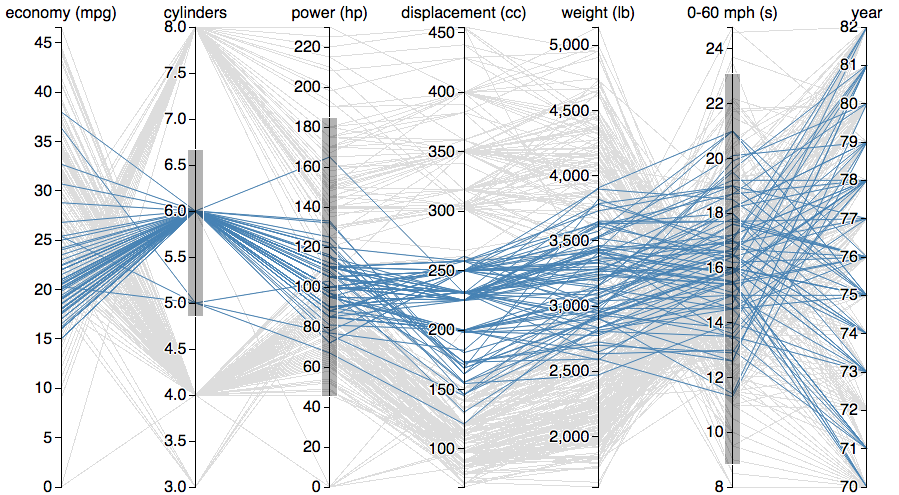
\includegraphics[width=\linewidth]{pcp}
	\caption{Direct manipulation in a parallel coordinates plot with reorder-able and brush-able axes.}
	\label{fig:lr-pcp}
\end{figure}

Another concept that can be applied to improve existing interaction techniques is \emph{fluid interaction}~\cite{Elmqvist2011}. Besides using direct manipulation as discussed previously, the interaction should produce smooth animated transitions between the state before and the state after an interaction, helping users maintain their mental maps; and provide immediate visual feedback, allowing users to know what is happening and/or what will happen next.

Typically, interaction techniques are combined to explore the data or present a known story. A classic visual information-seeking mantra by Shneiderman~\cite{Shneiderman1996} summarizes many design guidelines and interaction techniques for designing information visualizations: \emph{Overview first, zoom and filter, then details-on-demand}. With large datasets, it it challenging to create an overview and provides cues for further exploration. A more suitable approach in this case is \emph{Search, show context, expand on demand}~\cite{VanHam2009}.

\subsubsection{Evaluation Methods}
A visualization, no matter how novel and interesting it is, needs to be evaluated to check whether it meets the design goals and supports the target users to complete the intended tasks. Evaluation has been a research topic in visualization when the field becomes more matured~\cite{Plaisant2004}. Excellent reviews of visualization evaluation with different perspectives include evaluation techniques~\cite{Carpendale2008}, scenarios~\cite{Lam2012} and design process~\cite{Munroe2009}.

In this section, we review the evaluation techniques based on the visualization design model by Munzner~\cite{Munroe2009}, helping address different concerns separately. The four levels include: explain the tasks and available data in the vocabulary of the problem domain, abstract them into domain-independent operations and data types, design visual encoding and interaction techniques to solve the abstract tasks, and develop algorithms to execute these techniques efficiently. Each level has its own \emph{threats} to validity and methods to address them. Two types of methods are distinguished: \emph{immediate} approaches can be done before inner levels are implemented, whereas \emph{downstream} approaches requires all inner levels are completed. The threats and evaluation methods are summarized in \autoref{fig:lr-nested-model}.

\begin{figure}[!htb]
	\centering
	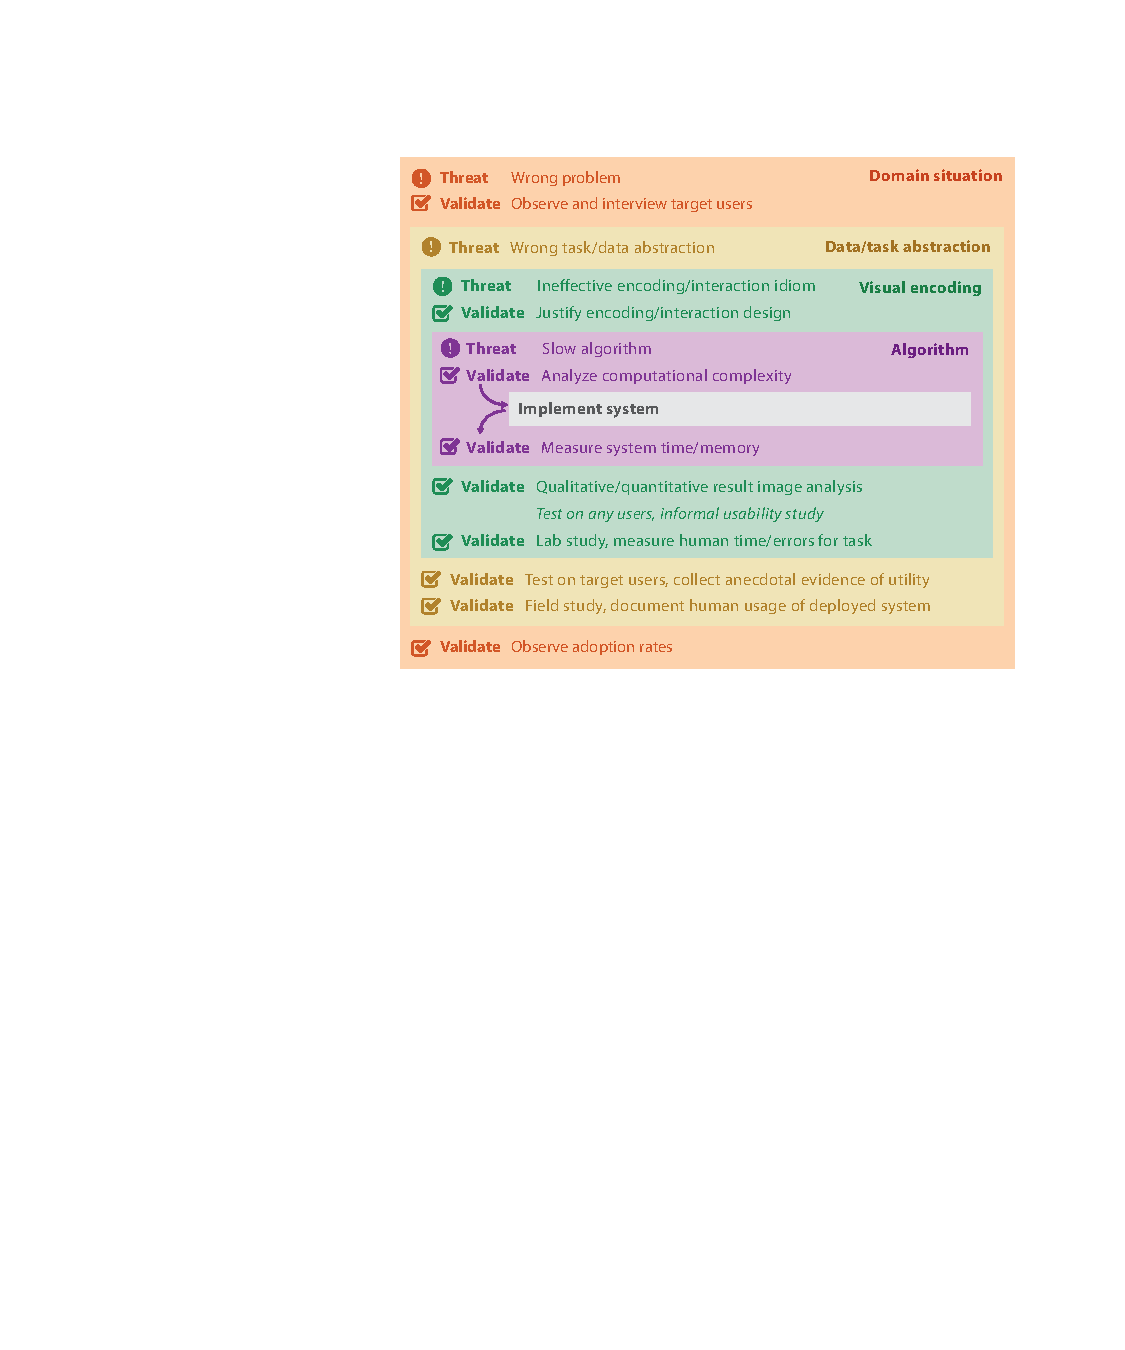
\includegraphics{nested-model}
	\caption{Threats and validation at each of the four nested levels of visualization design. \is{Munzner2014}}
	\label{fig:lr-nested-model}
\end{figure}

\paragraph{Domain Problem and Data Characterization}
The domain problem of target users is investigated to see if visualization is a potential solution. The primary threat is that the problem is mischaracterized: the users do not really suffer from the identified problem. An immediate form of validation is \emph{field study}~\cite{Carpendale2008}, where the investigator observes how target users act in real-world settings in order to learn and verify the characterization. Another technique is \emph{contextual inquiry}~\cite{Holtzblatt1993}, which allows the investigator to occasionally interview while the user is engaged in the process. One example is the study by Sedlmair~et~al.~\cite{Sedlmair2008} on current working behavior and environments of analysis and diagnosis experts in the automotive industry.

One downstream form of validation is to report the rate the adoption rate of the tool by the target users. High effort is required to make the visualization solution reliable and deployable in the real-world environment. Examples include a field study of Google's Notebook product~\cite{Russell2008} and 6-week field trial of SparTag.us -- a tagging system for foraging web content~\cite{Hong2008}.

\paragraph{Operation and Data Type Abstraction}
The threat at this level is the identified data and task abstraction do not solve the characterized problem. Only downstream approaches can be used to validate the abstraction. The deployed system needs to be used by target users completing their routine tasks in real-world environment. The goal of this evaluation is to collect anecdotal evidence that the solution is in fact useful. The observation and interview need to focus on understanding how the tool is used, and how it helps or hinders the users in performing their tasks. An example is a longitudinal field study of LiveRAC system that supports analysis of system management time-series data~\cite{McLachlan2008}.

Evaluating the visualizations for supporting sensemaking can be done at this level, as the \emph{evaluating visual data analysis and reasoning} scenario in the taxonomy by Lam~et~al.~\cite{Lam2012}. Due to the nature of sensemaking, evaluation is often carried out as case studies~\cite{Kang2011} with observation and interview, and followed by qualitative data analysis~\cite{Lazar2010}. Attempts also have been made to quantify the insight or knowledge gained during sensemaking~\cite{Wilson2013}.

\paragraph{Visual Encoding and Interaction Design}
At the design level, the threat is the chosen design is ineffective at communicating the desired abstraction to the user. One immediate form of validation is to justify every design decision based on known design principles such as the ones discussed in \autoref{sub:lr-design}, or more comprehensive predefined guidelines as in heuristic evaluation~\cite{Zuk2006}. Asking experts to review the design prototype also provides valuable feedback~\cite{Tory2005}.

A common downstream approach is to conduct a controlled experiment comparing the design with other state-of-the-art alternatives~\cite{Xu2012}. A number of participants, depending on the  expected size of the experiment, carry out a number of tasks representing real-world cases. Typically, task completion time and accuracy are measured and analyzed using hypothesis testing methods~\cite{Field2003}. Post-task interviews are often combined to establish deeper understanding about how the visualization is used. If the experiment can be completed online, crowd-sourcing approach using Amazon's Mechanical Turk service can help largely increase the size of participants~\cite{Heer2010a}. Another downstream approach is the measurement of common aesthetic metrics such as the number of edge crossings and edge bends that have been used in graph visualization~\cite{Sugiyama1981}.

\paragraph{Algorithm Design}
The primary threat at this level is the algorithm is suboptimal in terms of time or memory performance. In interactive visualization, it is essential to ensure the interaction responsive in real-time. Analyzing the complexity of the algorithm using the standard approaches from the computer science literature~\cite{Cormen2009} is an intermediate form of validation. The complexity can be computed based on the size of dataset or the display screen. Downstream approaches include measuring running time and memory usage for benchmark datasets.













%http://www.cc.gatech.edu/~stasko/papers/vast09-eval.pdf
%https://www.purdue.edu/discoverypark/vaccine/assets/pdfs/publications/pdf/Beyond%20Usability.pdf
%http://www.cc.gatech.edu/~stasko/7450/Papers/fekete08.pdf
%https://www.cs.ubc.ca/~tmm/courses/cpsc533c-05-fall/readings/vov.pdf